% -------------------------------------------------------------------------------------------------
%
%  Skeleton for semester and master thesis reports at the Laboratory for Software Technology.
%  Based on the skeleton provided by the Institute of Robotics and Intelligent Systems.
%
% -------------------------------------------------------------------------------------------------
%
% USAGE:      compile with PDFLaTeX
%
% HISTORY:    - written by Sascha A. Stoeter <stoeter@iris.ethz.ch>, www.stoeter.com, 02.06.2004
%             - modified by Martin Probst, 18.08.2004
%             - extended and adapted for use at LST by Oliver Trachsel, 2007-08-21
% -------------------------------------------------------------------------------------------------
\documentclass[11pt,a4paper]{book}
\usepackage{lstreport}

% -------------------------------------------------------------------------------------------------
% Add needed packages. Some generally useful packages are listed for
% your convenience.
% -------------------------------------------------------------------------------------------------
\usepackage{subfigure}                          % enable the use of subfigures
\usepackage[thickspace,thinqspace]{SIunits}     %
\usepackage[plainpages=false,pdfpagelabels]{hyperref}    % enable hyperlinks in pdf/ps Docs
\usepackage{listings}                           % to embed source code


% UTF8
\usepackage[utf8x]{inputenc} 

% -------------------------------------------------------------------------------------------------
% Select type of thesis
% -------------------------------------------------------------------------------------------------
\renewcommand{\thesistype}{Bachelor}
%\renewcommand{\thesistype}{Diploma}
%\renewcommand{\thesistype}{Master}

% -------------------------------------------------------------------------------------------------
% Set names
% -------------------------------------------------------------------------------------------------
\renewcommand{\thesisauthor}{Marcel Mohler}
\renewcommand{\thesisadvisor}{Zoltán Majó \\ Tobias Hartmann}

%OWN STUFF###############################################################
\usepackage[english]{babel}

% colors
%\definecolor{orange}{rgb}{1,0.5,0}

% Disable single lines at the start of a paragraph (Schusterjungen)

\clubpenalty = 10000

% Disable single lines at the end of a paragraph (Hurenkinder)

\widowpenalty = 10000
\displaywidowpenalty = 10000
 
% allows for colored, easy-to-find todos

\newcommand{\todo}[1]{\textsf{\textbf{\textcolor{orange}{[[TODO: #1]]}}}}


%##########################################################################


% -------------------------------------------------------------------------------------------------
% Beginning of the main document body
% -------------------------------------------------------------------------------------------------
\begin{document}

% include all bibtex even if not cited
\nocite{*}

% -------------------------------------------------------------------------------------------------
% Front matter with title page, table of contents, and abstracts 
% -------------------------------------------------------------------------------------------------
\frontmatter

% Title page: set title and date 
\thesistitlepage{Profile Caching for the\\Java Virtual Machine
}{August 2015}

% Abstract must not be longer than one page per language. English and
% German abstracts are mandatory.
\chapter*{Introduction}
\label{s:Introduction}
Virtual machines (VMs) like the Java Virtual Machine (JVM) are used as the execution environment of choice for many modern programming languages. 
VMs interpret a suitable intermediate language (e.g., Java Byte Code for the JVM) and provide the runtime system for application programs. VMs usually include a garbage collector, a thread scheduler, and interfaces to the host operating system. 
As interpretation of intermediate code is time-consuming, VMs usually include a \textit{Just-in-time} (JIT) compiler that translates frequently-executed functions or methods to \textit{native} machine code.
\\\\
The JIT compiler executes in parallel to a program's interpretation by the VM and, as a result, compilation speed is a critical issue in the design of a JIT compiler.
Unfortunately, it is difficult to design a compiler such that the compiler produces good or excellent code while limiting the resource demands of this compiler. The compiler requires storage, CPU cycles and even on a multi-core processor, compilation may slow down the execution of the application program.
\\\\
Consequently, most VMs adopt a multi-tier compilation system.
%The first tier usually is the interpretation of a method. If this method is executed frequently, the Tier-1 compiler translates this method into native code.
%The Tier-1 compiler implements only a small set of the know optimization techniques and as result, it had good compilation speed but the generated code is far from the output of an optimizing compiler. Such a compiler is usually the Tier-2 compiler, which takes a longer amount of time and produces optimized native code. To determine which methods should be compiled by the Tier-1 (or Tier-2) compiler, the VM profiles the execution of all application programs to identify “hot” methods.
At program startup, all methods are interpreted by the virtual machine (execution at Tier 0). The interpreter gathers execution statistics called \textit{profiles} and if a method is determined to be executed frequently, this method is then compiled by the Tier 1 compiler. Methods compiled to Tier 1 are then profiled further and based on these profiling information, some methods are eventually compiled at higher tiers.
One of the drawbacks of this setup is that for all programs, all methods start in Tier 0, with interpretation and profiling by the VM. However, for many programs the set of the most used methods does not change from one execution to another and there is no reason to gather profiling information again. 
\\\\
The main idea of this thesis is to cache these profiles from a prior execution to be used in further runs of the same program. 
Having these \textit{cached profiles} available avoids the JIT compiler to gather the same profiling information again. As well as allow the compiler to use more sophisticated profiles early in program execution and prevent recompilations when more information about the method is available. While this in general should not significantly influence the peak performance of the program, the hope is to decrease the time the JVM needs to achieve it, the so called \textit{warmup}.
\\\\
This thesis proposes a design and an implementation of a profile caching feature for \textit{HotSpot}, an open source Java virtual machine maintained and distributed by Oracle Corporation as well as a profound performance analysis using state-of-the-art benchmarks.


%\chapter*{Zusammenfassung}
%Kurzfassung der Arbeit.

% Table of contents
\tableofcontents

% -------------------------------------------------------------------------------------------------
% Main document body
% -------------------------------------------------------------------------------------------------
\mainmatter
\chapter{Motivation}
\label{s:Motivation}
I continue with presenting two very simple example methods that illustrate the motivation and benefit from using cached profiles.
This should provide the reader with an understanding how and why cached profiles can be beneficial for the performance of a Java Virtual Machine.
I will omit any implementation details on purpose as they will be discussed in Chapter \ref{c:implementation} in detail.
\\\\
Ideally, being able to reuse the profiles from previous runs should result in two main advantages:
\begin{enumerate}
  \item \textbf{Lower start-up time of the JVM:} Having information about the program flow already, the compiler can avoid gathering profiles and compile methods earlier and directly at higher compilation levels.
  \item \textbf{Less Deoptimizations:} Since cache profiles get dumped at the end of a compilation, when using these profiles the compiler can already include all optimizations for all different method executions. Less uncommon traps need to be placed and less deoptimizations occur.
\end{enumerate}
\begin{figure}[ht]
  \begin{center}
    \centering
    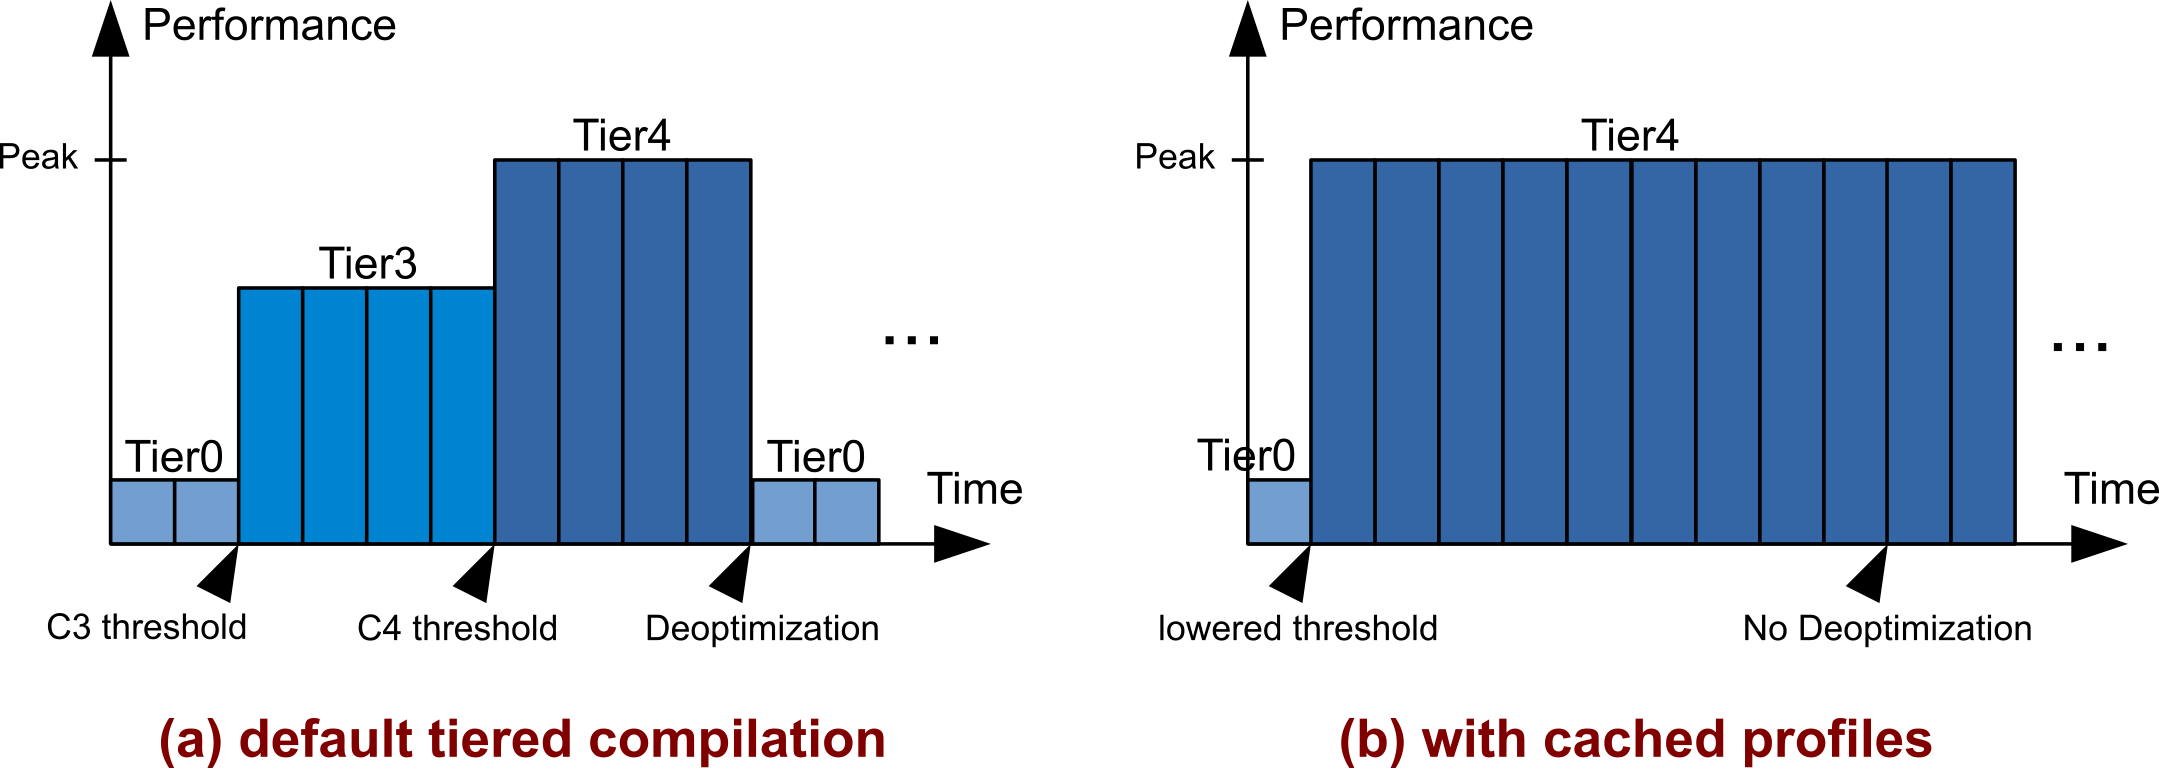
\includegraphics[width=0.9\textwidth]{figures/baseline_vs_usage.png}
    \caption{schematic visualization of cached profile benefit}
    \label{f:baseline_vs_usage}
  \end{center}
\end{figure}
Figure \ref{f:baseline_vs_usage} gives a schematic visualization of the expected effect on performance of a single method when using cached profiles compared to the current state without such a system and standard tiered compilation.
The blue bars roughly represent method invocations and higher bars equal higher compilation levels and therefore higher performance. The x-axis represents time since the start of the JVM. The figure shows the ideal case and abstracts away many details and other possible cases. However, it provides a good visualization for the examples provided in this chapter. A more detailed performance analysis, also considering worse cases is done in Chapter \ref{c:performance}.
\\\\
I'm using my implementation described in Chapter \ref{c:implementation} in CachedProfileMode 0 (see \ref{s:mode0}) built into openJDK 1.9.0.
All measurements in this chapter are done on a Dual-Core machine running at 2 GHz with 8GB of RAM. To measure the method invocation time I use hprof \cite{hprof} and the average of 10 runs. The evaluation process has been automated using a couple of python scripts. The error bars show the 95\% confidence interval.
\section{Example 1}
\label{s:ex1}
For this very first example, on-stack replacement has been disabled to keep the system simple and easy to understand.
\\
Example one is a simple class that invokes a method one hundred times. The method itself consists of a long running loop. The source code is shown in Listing \ref{l:nocompile}.
Since OSR is disabled and a compilation to level 3 is triggered after 200 invocations this method never leaves the interpreter. I call this run the \textit{Baseline}.
To show the influence of cached profiles I use a compiler flag to lower the compile threshold explicitly and, using the functionality written for this thesis, tell Hotspot to cache the profile.
In a next execution I use these profiles and achieve significantly better performance as one can see in Figure \ref{f:nocompile}.
This increase comes mainly from the fact that having a cached profile available allows the JVM to compile highly optimized code for hot methods earlier (at a lower threshold) since there is no need to gather the profiling information first.
\\
Since the example is rather simple neither the baseline nor the profile usage run trigger any deoptimization. This makes sense because after the first invocation, all the code paths of the method have been taken already and are therefore known to the interpreter and saved in the profile.
\begin{lstlisting}[float,caption=Simple method that does not get compiled,label=l:nocompile,language=Java]
class NoCompile {
    double result = 0.0;
    for(int c = 0; c < 100; c++) {
      result = method1(result);
    }
    public static double method1(double count) {
        for(int k = 0; k < 10000000; k++) {
            count = count + 50000;
        }
        return count;
   }
}
\end{lstlisting}
\begin{figure}[ht]
  \begin{center}
    \centering
    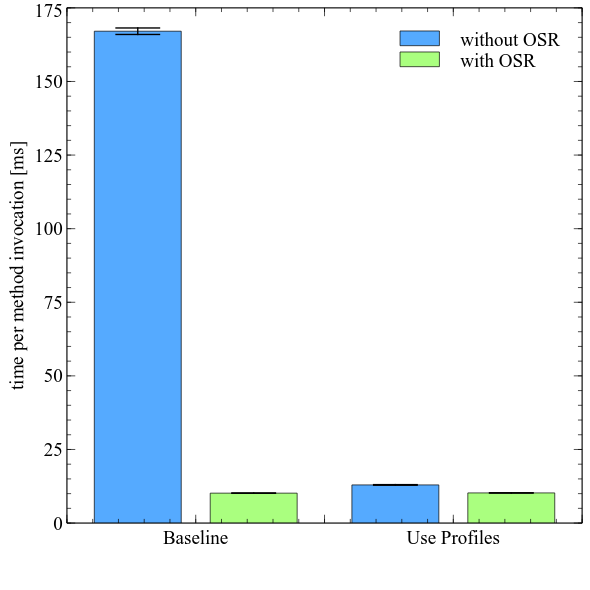
\includegraphics[width=0.5\textwidth]{figures/nocompile.png}
    \caption{NoCompile.method1 - per method invocation time}
    \label{f:nocompile}
  \end{center}
\end{figure}
\\
Enabling OSR again and the difference between with and without cached profiles vanishes.
This happens because Hotspot quickly realizes the hotness of the method and the JIT compiler produces perfectly optimized code during the first method invocation already. 
Even the OSR compiled code never triggers any deoptimization due to the simplicity of the loop.
So this example appears rather artificial since the same performance can be achieved with OSR already but nevertheless shows the influence of early compilation.
\section{Example 2}
\label{s:ex2}
However, OSR is one of the main features of Hotspot to improve the JIT performance and disabling that does not give us any practical results. Since we want an example which demonstrates the influence of cached profiles, I came up with the example sketched in Listing \ref{l:manydeopts} which is slightly more complex but still easy to understand.
\\\\
The idea is to create a method that takes a different, long running branch on each of it's method invocations. Each branch has been constructed in a way that it will trigger an OSR compilation. When compiling this method during its first iteration only the first branch will be included in the compiled code. The same will happen for each of the 100 method invocations. As one can see in Figure \ref{f:manydeopts} the baseline indeed averages at around 130 deoptimizations and a time per method invocation of 200 ms.
\\\\
Now I use a regular execution to dump the profiles and then use these profiles. So theoretically the profiles dumped after a full execution should include knowledge of all branches and therefore the compiled method using these profiles should not run into any deoptimizations. As one can see in Figure \ref{f:manydeopts} this is indeed the case. When using the cached profiles no more deoptimizations occur and because less time is spent profiling and compiling the methods the per method execution time is even significantly faster with averaging at 190ms now.
\begin{lstlisting}[float,caption=Simple method that causes many deoptimizations,label=l:manydeopts,language=Java]
class ManyDeopts {
    double result = 0.0;
    for(int c = 0; c < 100; c++) {
      result = method1(result);
    }
    public static long method1(long count) {
        for(int k = 0l; k < 10000000l; k++) {
            if (count < 10000000l) {
                count = count + 1;
            } else if (count < 30000000l) {
                count = count + 2;
                .
                .
                .
            } else if (count < 50500000000l) {
               count = count + 100;
            }
            count = count + 50000;
        }
        return count;
   }
}
\end{lstlisting}
\\\\\\\\\\\\
\begin{figure}[ht!]
  \begin{center}
    \centering
    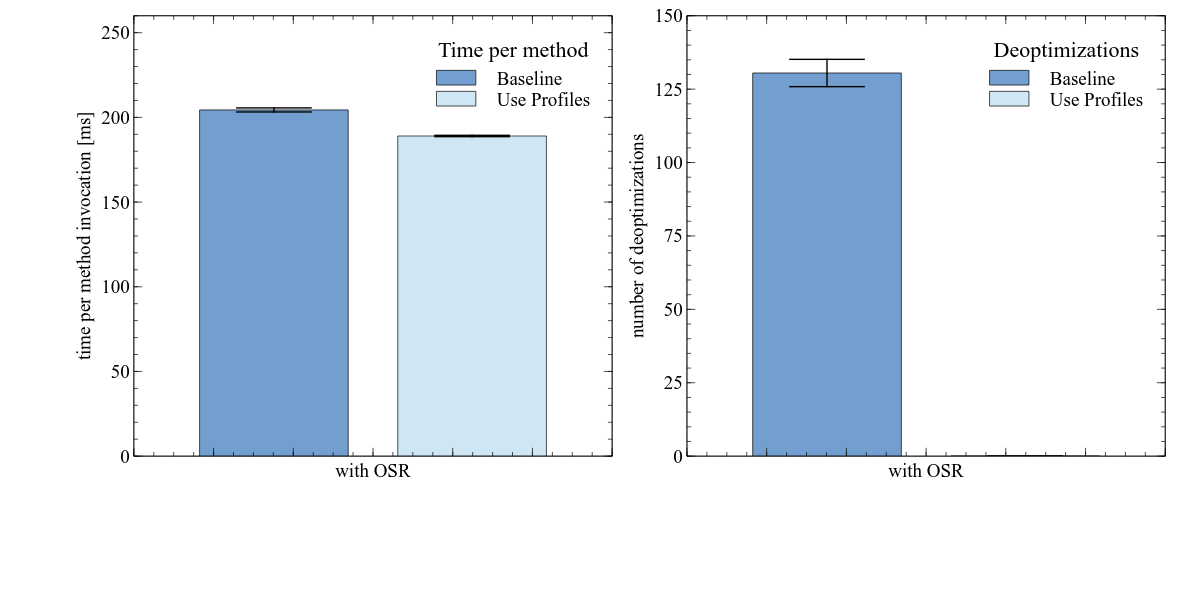
\includegraphics[width=0.9\textwidth]{figures/manydeopt.png}
    \caption{ManyDeopts.method1 - per method invocation time and deoptimization count}
    \label{f:manydeopts}
  \end{center}
\end{figure}
\\\\
\section{Similar systems}
\label{s:similarsystems}
In commercially available JVMs the idea of caching profiles is not new.
In fact the JVM developed and sold by Azul Systems\textregistered\ called Zing\textregistered\ \cite{zing} already offers a similar functionality.
Zing\textregistered\ includes a feature set they call ReadyNow!\texttrademark\ \cite{readynow} that aims to increase warmup performance of Java applications.
Their system has been designed with financial markets in mind and to overcome the issue of slow performance in the beginning and performance drops during execution.
Azul Systems clients reported that their production code usually experiences a significant performance drop as soon as the market goes live and the clients start trading.
The reasons are deoptimizations that occur because due to changed situation uncommon branch paths are taken or yet unused methods are invoked.
In the past their clients used techniques to warm up the JVM, for example doing fake trades. However this does not solve the problem since the JVM optimizes for these fake trades and still runs into deoptimizations once actual trades are meant to happen.
\\\\
ReadyNow!\texttrademark\  is a rich set of improvements how a JVM can overcome this issues. It includes attempts to reduce the number of deoptimizations in general and other not further specified optimizations.
As one of the core features Azul Systems\textregistered\ implemented the ability to log optimization statistics and decisions and reuse this logs in future runs. This is similar to the approach presented in this thesis. However they do not record the actual optimization but the learning and the reasons why certain optimizations happen. This gives them the ability to give feedback to the user of the JVM whether or not certain optimizations have been applied. They also provide APIs for developers to interact with the system and allow further fine-grained custom-designed optimizations.
\\\\
Unfortunately, they do not provide any numbers how their system actually improves performance.


\chapter{Implementation / Design}
\label{s:implementation}
This chapter describes the implementation of the cached profiles implementation for Hotspot, written as part of this thesis.
\\\\
Hotspot is an Java virtual machine implementation maintained by Oracle Cooperation. It is part of the open source project \texttt{OpenJDK} and the source code is available at \url{http://openjdk.java.net/}.
\\\\
Most of the work is included in two new classes \texttt{/share/vm/ci/ciCacheProfiles.cpp} and \\\texttt{/share/vm/ci/ciCacheProfilesBroker.cpp} as well as modifications to \texttt{/share/vm/ci/ciEnv.cpp} and \texttt{/share/vm/compiler/compileBroker.cpp}.
\\
Most of the code is located in \texttt{/share/vm/ci/ciCacheProfiles.cpp}, a class that takes care of setting up a datastructure for the cached profiles as well as providing public methods to check if a method is cached or not. The class \texttt{/share/vm/ci/ciCacheProfilesBroker.cpp} gets called before a method that has a profile available gets compiled. It is responsible for setting up the compilation environment so the JIT compiler can use the cached profiles.
\\\\
A full list of modified files and the changes can be seen in the webrev or appendix TODO.
\\\\
The changes are provided in form of a patch for Hotspot version 8182 TODO. This original version is referred to as \textit{Baseline}.
\\\\
I will describe and explain the functionality and the implementation design decision in the following sections, ordered by the appearance in execution.


\section{Creating cached profiles}
\label{s:creatingprofiles}
The baseline version of Hotspot already offered a functionality to replay a compilation based on dumped profiling information.
This is mainly used in case the JVM crashes during JIT compilation to replay the compilation again and help finding the cause of this crash.
Dumping the data needed for the replay is either be done automatically in case of a crash or can be invoked manually by specifying the \texttt{DumpReplay} compile command option per method.
I introduce method option called \texttt{DumpProfile} as well as a compiler flag \texttt{-XX:+DumpProfiles} that appends profiling information to a file as soon as the method gets compiled. The first option can be specified as part of the \texttt{-XX:CompileCommand} or \texttt{-XX:CompileCommandFile} flag and allows one to force single methods to dump their profile. The second commands dumps all profiles of all compiled methods into a single file called \textit{cached\_profiles.dat}.
\\\\
As soon as a method gets compiled all information about the methods used in the compiled method as well as their profiling information get converted to a string and written to disk. Since method often get compiled multiple times this can result in dumping compilation information about the same method multiple times. How this will be taken care of is described in Section \ref{s:initializingprofiles}
Together with some additional information about the compilation itself, for example the bytecode index of the compiled method in case of OSR, the compiler will be able to redo the same compilation on a future run of the java virtual machine.  
\section{Initializing cached profiles}
\label{s:initializingprofiles}
I introduce a new compiler flag \texttt{-XX:+CacheProfiles} that enables the use of profiles that have been written to disk in a previous run of the Java Virtual Machine. Per default it reads from a file called \textit{cached\_profiles.dat} but a different file can be specified using \\\texttt{-XX:CacheProfilesFile=other\_file.dat}.
\\\\
Before any cached profiles can be used the virtual machine has to parse that file and organize the profiles and compile information in a simple datastructure. This datastructure is kept in memory during the whole execution of the JVM to avoid multiple scans of the file.
The parsing process gets invoked during boot up of the JVM, directly after the compileBroker gets initialized. This happens before any methods get executed and blocks the JVM until finished.
As mentioned in Section \ref{s:creatingprofiles} the file consists of method informations, method profiles and additional compile information. The parser scans the file once and creates a so called \texttt{CompileRecord} for each of the methods that include compilation information in the file. This compile record also includes the list of method information and their profiling information.
A method's compile information could have been dumped multiple times, so it can happen that there are multiple CompileRecords for the same method. In this case, Hotspot will only keep the CompileRecords that are created based on the data written to the file last.
Since profiling information only grow, the compilation that happened last contains the richest profile and is considered the best to avoid deoptimizations.
\\\\
The CompileRecord as well as the lists of methods information and profiles are implemented as an array located in Hotspot's heap space.
They get initialized with a length of 8 and grow when needed. The choice has been done for simplicity and leaves up room for further optimizations.

\section{Using cached profiles}
\label{s:usingprofiles}
The idea is to use cached profiles whenever possible and if none are available continue as usual.
A graphical, simplified overview of the program flow for compiling a method with the changes introduced in this thesis can be found in Figure \ref{f:programflow}.
\begin{figure}[h]
  \begin{center}
    \centering
    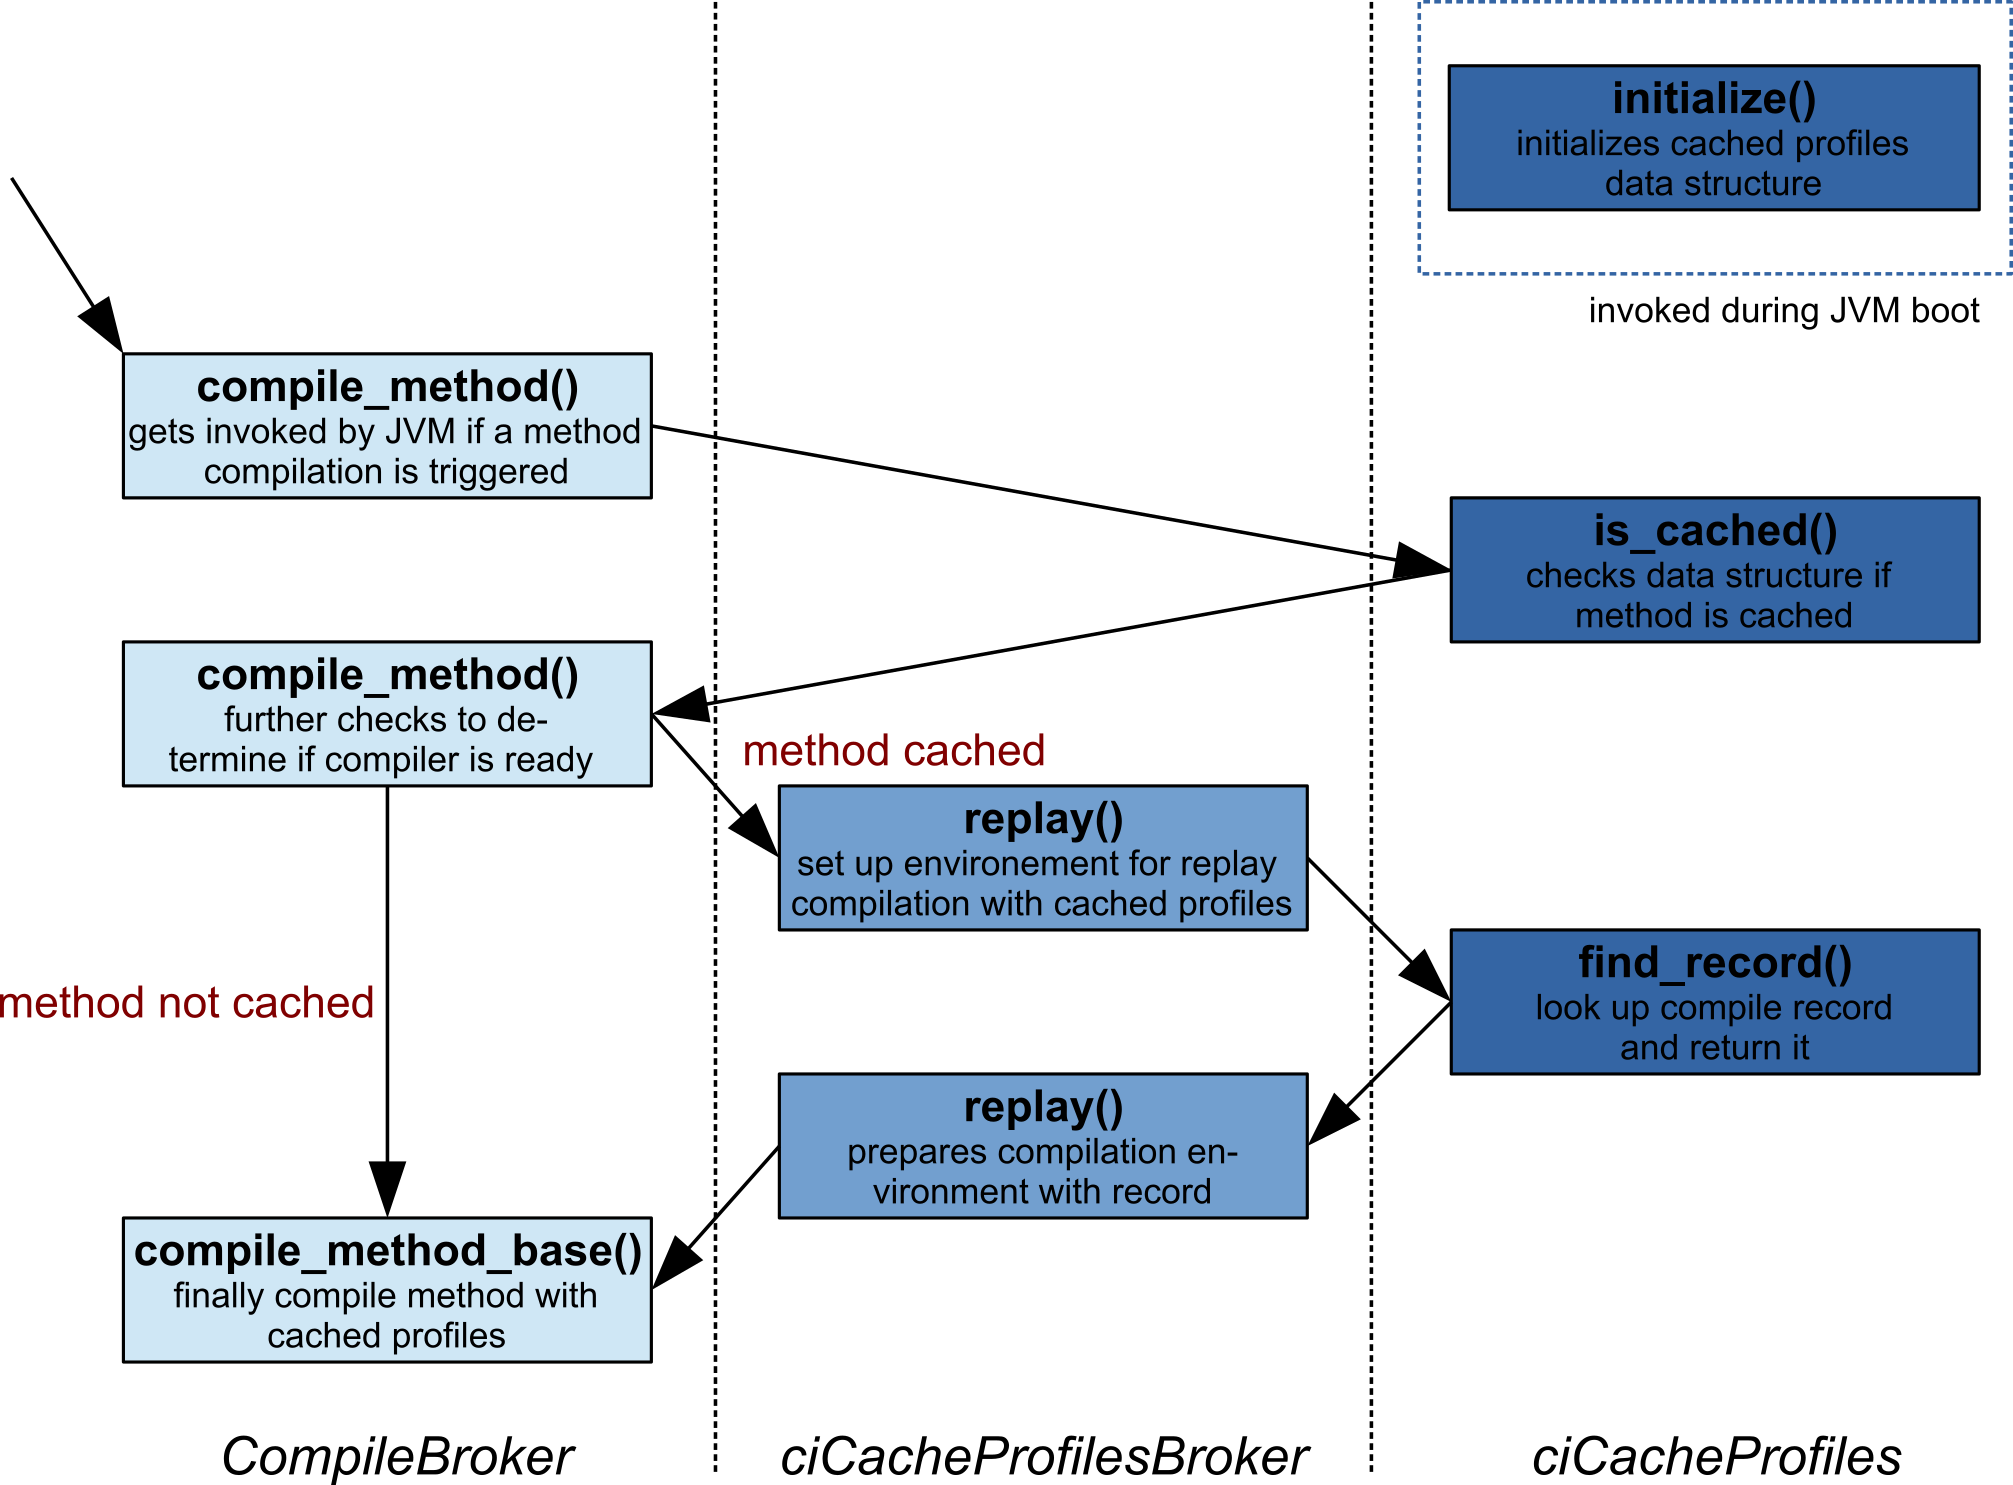
\includegraphics[width=0.8\textwidth]{figures/program_flow.png}
    \caption{program flow for compiling a method}
    \label{f:programflow}
  \end{center}
\end{figure}
As mentioned before once certain thresholds are exceeded a method gets scheduled for compilation. This means that the JVM will invoke a method called \texttt{compile\_method()} located in the \texttt{compileBroker} class. This method for example checks if the compile queue isn't full or if there is already another compilation of that particular method running.
I extended this method with a call to \texttt{ciCacheProfiles::is\_cached(Method* method)} which either returns 0 if the method is not cached or returns an integer value, reflecting the compile level, in case that method has a cached profile available.
In case the method is not cached the execution continues as in the baseline.
Otherwise the compileBroker will call into \texttt{ciCacheProfilesBroker} to replay the compilation, based on the saved profile.

\section{Different usage modes for cached profiles}
The implementation of cached profiles offers 3 different modes how
\label{s:cacheprofilesmode}
\subsection{Compile Thresholds lowered (mode 0)}
\label{s:mode0}
\subsection{Unmodified Compile Thresholds (mode 1)}
\label{s:mode1}
\subsection{Modified C1 stage (mode 2)}
\label{s:mode2}

\section{Debug outout}
\label{s:debugoutput}
For debugging and benchmarking purposes I implemented four debug flags that can be used along with \texttt{-XX:+CacheProfiles}.
-XX:+PrintCacheProfiles
-XX:+PrintDeoptimizationCount
-XX:+PrintDeoptimizationCountVerbose
-XX:+PrintCompileQueue


\chapter{Performance}
\label{s:Performance}
\section{Examples}

\section{SPECjvm 2008}

\section{Nashorn / Octane}


\chapter{Conclusion}
\label{s:Conclusion}
Modern Java Virtual Machines (JVM) like HotSpot gather profiling information about executed methods to improve the quality of the compiled code.
This thesis presents several approaches to reuse profiling information, that has been dumped to disk in previous executions of the JVM.
\\\\
The expected advantage is a faster warmup of the Java Virtual Machine, because the JVM does not need to spend time profiling the code and can use cached profiles directly.
Furthermore, since the cached profiles originate from previous compilations, where extensive profiling already happened, compilations using these profiles produce more optimized code, which decreases the amount of deoptimizations.
\\\\
We show, using two benchmark suites, that cached profiles can indeed improve warmup performance and significantly lower the amount of deoptimizations as well as reduce the time spent in the JIT compilers.
Therefore, we believe that cached profiles are a valuable asset in scenarios where a fast JVM warmup is needed and performance fluctuations at runtime should be avoided.
\\\\
In addition, we evaluated the performance of our approach with individual benchmarks for the impact of cached profiles on the load of the compile queue and the amount and type of compilations. The results show, that neither of them gives one-to-one correspondence between the examined factor and performance. However, the results provide indications, where the performance increase or decrease could come from.
\\\\
The functionality is implemented in the HotSpot JVM (OpenJDK9). Several new HotSpot options are added to allow fine tuning of the system, including the possibility to selectively enable or disable profile caching.

% -------------------------------------------------------------------------------------------------
% Appendices (if needed)
% -------------------------------------------------------------------------------------------------
\appendix
\chapter{Extra Stuff}
\label{s:ExtraStuff}

Additional material such as long mathematical derivations.

% -------------------------------------------------------------------------------------------------
% Bibliography
% -------------------------------------------------------------------------------------------------
\addcontentsline{toc}{chapter}{Bibliography}
\bibliography{bibliography}

\end{document}
